\documentclass[noinstructornotes]{ximera}
%handout:  for handout version with no solutions or instructor notes
%handout,instructornotes:  for instructor version with just problems and notes, no solutions
%noinstructornotes:  shows only problem and solutions

%% handout
%% space
%% newpage
%% numbers
%% nooutcomes

%I added the commands here so that I would't have to keep looking them up
%\newcommand{\RR}{\mathbb R}
%\renewcommand{\d}{\,d}
%\newcommand{\dd}[2][]{\frac{d #1}{d #2}}
%\renewcommand{\l}{\ell}
%\newcommand{\ddx}{\frac{d}{dx}}
%\everymath{\displaystyle}
%\newcommand{\dfn}{\textbf}
%\newcommand{\eval}[1]{\bigg[ #1 \bigg]}

%\begin{image}
%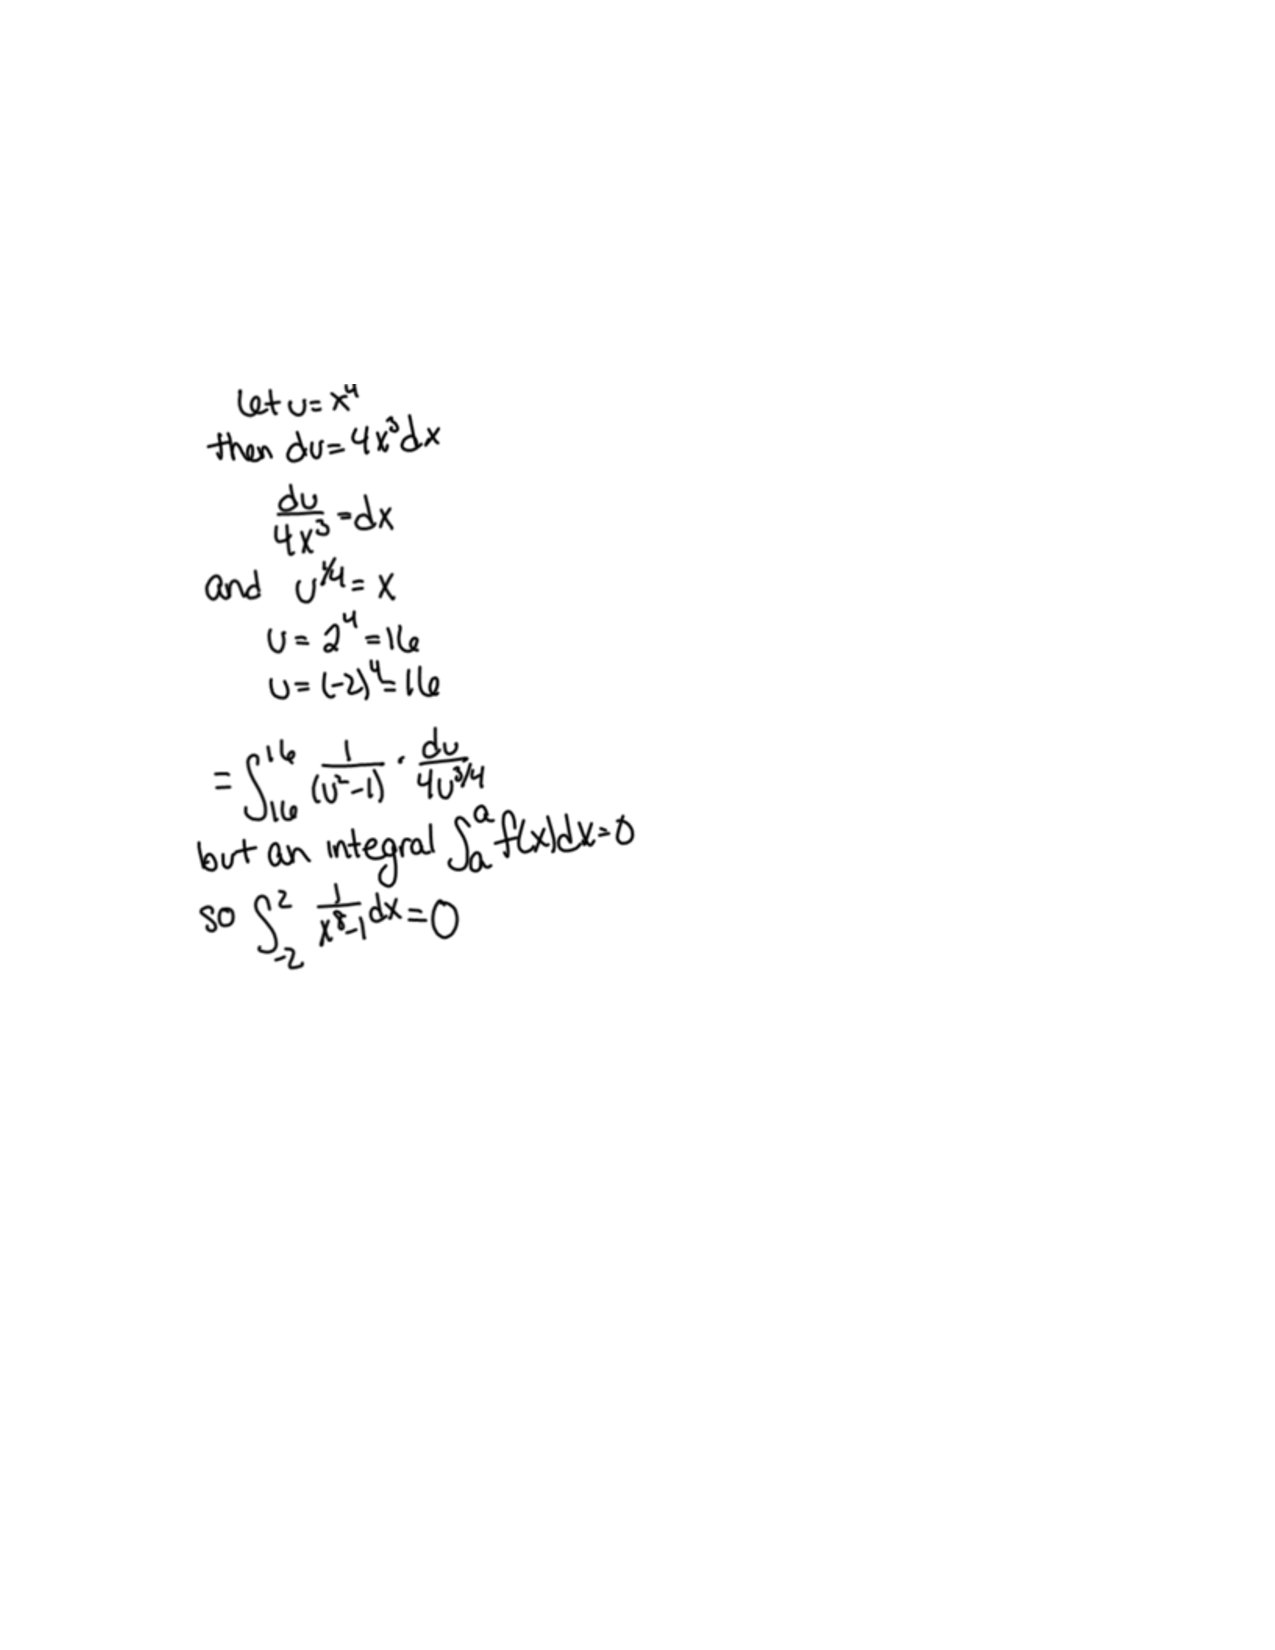
\includegraphics[trim= 170 420 250 180]{Figure1.pdf}
%\end{image}

%add a ``.'' below when used in a specific directory.
\newcommand{\RR}{\mathbb R}
\renewcommand{\d}{\,d}
\newcommand{\dd}[2][]{\frac{d #1}{d #2}}
\renewcommand{\l}{\ell}
\newcommand{\ddx}{\frac{d}{dx}}
\newcommand{\dfn}{\textbf}
\newcommand{\eval}[1]{\bigg[ #1 \bigg]}

\usepackage{multicol}

\renewenvironment{freeResponse}{
\ifhandout\setbox0\vbox\bgroup\else
\begin{trivlist}\item[\hskip \labelsep\bfseries Solution:\hspace{2ex}]
\fi}
{\ifhandout\egroup\else
\end{trivlist}
\fi} %% we can turn off input when making a master document

\title{Recitation \#10: Trig Substitution and Partial Fractions}  

\begin{document}
\begin{abstract}		\end{abstract}
\maketitle



\begin{comment}
\section{Warm up:}

	\begin{freeResponse}
	
	\end{freeResponse}
	
\begin{instructorNotes}

\end{instructorNotes}
\end{comment}







\section{Group work:}



%problem 1
\begin{problem}
Without determining the coefficients, write the partial fraction decomposition of the following rational function:
	\[
	\frac{5x^{13} - 6x^{12} + 7x^3 - 5x - 18}{(2x-3)(5x+9)^3 (x^2+9x+19)(x^2+9x+21)^2}
	\]
	\begin{freeResponse}
	The degree of the numerator is $13$, whereas the degree of the denominator is $10$.  
	So if we perform long division, we will get a degree $13-10=3$ polynomial plus partial fractions for the remainder term:
		\begin{align*}
		&\frac{5x^{13} - 6x^{12} + 7x^3 - 5x - 18}{(2x-3)(5x+9)^3 (x^2+9x+19)(x^2+9x+21)^2} = Ax^3 + Bx^2 + Cx + D  \\
		&+ \frac{E}{2x-3} + \frac{F}{5x+9} + \frac{G}{(5x+9)^2} + \frac{H}{(5x+9)^3} + \frac{I}{x-i_1} + \frac{J}{x-i_2}  \\
		&+ \frac{Kx+L}{x^2+9x+21} + \frac{Mx+N}{(x^2+9x+21)^2}.
		\end{align*}
		
	\dfn{Explanation of $i_1$ and $i_2$:} 
	The quadratic $x^2+9x+19$ can be factored over the real numbers, since the discriminant $b^2-4ac = 81-76 > 0$.  
	The numbers $i_1$ and $i_2$ are the two real roots to this polynomial, ie
		\[
		i_1 = \frac{-9+\sqrt{5}}{2}	\qquad	i_2=\frac{-9 - \sqrt{5}}{2}.
		\]
	Note that the polynomial $x^2+9x+21$ is irreducible (over the real numbers) since its discriminant is less than $0$.  
	\end{freeResponse}
	
\end{problem}

\begin{instructorNotes}
Make sure that the students do not attempt to perform the long division.  
We are only looking for the \dfn{form} of the decomposition, which will be a cubic polynomial followed by a sum of rational functions.  
Note that $x^2 + 9x +19$ can be factored over the reals while $x^2 + 9x + 21$ cannot.  
This is a good time to talk about the descriminant.
\end{instructorNotes}







%problem 2
\begin{problem}
Evaluate:
	\[
	\int \frac{7x^3 + 18x + 9}{x^4 + 9x^2} \d x
	\]
{\it Hint:  If $f(x) = 7x^3 + 18x + 9$, then $f(2) = 101$, $f(1) = 34$, and $f(-1) = -16$.}
	\begin{freeResponse}
	First factor the denominator
		\[
		x^4 + 9x^2 = x^2(x^2 + 9).
		\]
	The we can decompose the integrand as a partial fraction
		\begin{equation*}
		\frac{7x^3+18x+9}{x^2(x^2+9)} = \frac{A}{x} + \frac{B}{x^2} + \frac{Cx+D}{x^2+9}
		\end{equation*}
		\begin{align*}
		\Longrightarrow	\quad	7x^3 + 18x + 9 &= Ax(x^2+9) + B(x^2+9) + (Cx+D)x^2  \\
		&= Ax^3 + 9Ax + Bx^2 + 9B + Cx^3 + Dx^2  \\
		&= (A+C)x^3 + (B+D)x^2 + 9Ax + 9B.
		\end{align*}
	By equating coefficients for powers of $x$ we have that
		\begin{align*}
		&9 = 9B 	\qquad	\Longrightarrow	\qquad	B = 1  \\
		&18=9A 	\qquad	\Longrightarrow	\qquad	A = 2  \\
		&0 = B+D 	\qquad	\Longrightarrow	\qquad	0 = 1 + D 	\qquad \Longrightarrow \qquad D = -1  \\
		&7=A+C 	\qquad	\Longrightarrow	\qquad	7=2+C 	\qquad \Longrightarrow \qquad C = 5.
		\end{align*}
	Thus
		\begin{align*}
		\int \frac{7x^3 + 18x + 9}{x^4 + 9x^2} \d x
		&= \int \left( \frac{2}{x} + \frac{1}{x^2} + \frac{5x-1}{x^2+9} \right) \d x  \\
		&= 2 \ln |x| - \frac{1}{x} + 5 \int \frac{x}{x^2 + 9} \d x - \int \frac{1}{x^2 + 9} \d x  \\
		&= 2 \ln |x| - \frac{1}{x} + \frac{5}{2} \ln (x^2 + 9) - \frac{1}{3} \arctan \left( \frac{x}{3} \right) + C.
		\end{align*}
	Note that, in the previous step, we substituted $u = x^2 + 9$ for the first integral and $u = \frac{x}{3}$ in the second integral.
	\end{freeResponse}
		
\end{problem}

\begin{instructorNotes}
First, note that students often have difficulty understanding that $x^2 = (x-0)^2$ is a perfect square of a linear factor $(x-0)$.  
The hint should help the students quickly solve for the unknowns.  
Using $x=0$ (not mentioned, but easily evaluated), one of the unknowns is immediately known.  
Using $1$ and $-1$ and adding the resulting equations finds a second unknown.  
Using $2$ will give them two equations and two unknowns to find the other two.  
The decomposition is
	\[
	\frac{2}{x} - \frac{1}{x^2} + \frac{5x-1}{x^2 + 9}.
	\]
\end{instructorNotes}




%problem 3
\begin{problem}
Evaluate the following integrals
	\begin{enumerate}

		
	\item 
	\[
	\int \frac{x^2}{\sqrt{4x-x^2}} \d x.
	\]
	\begin{freeResponse}
	Again, we begin by completing the square in the denominator, and then factoring
		\begin{align*}
		4x-x^2 &= -(x^2-4x)  \\
		&= -(x^2-4x+4) + 4  \\
		&= -(x-2)^2 + 4  \\
		&= 4 \left( - \frac{(x-2)^2}{4} + 1 \right)  \\
		&= 4 \left( 1 - \left( \frac{x-2}{2} \right)^2 \right).
		\end{align*}
	So
		\begin{align*}
		\int \frac{x^2}{\sqrt{4x-x^2}} \d x &= \int \frac{x^2}{\sqrt{4 \left( 1 - \left( \frac{x-2}{2} \right)^2 \right)}} \d x  \\
		&= \frac{1}{2} \int \frac{x^2}{\sqrt{1 - \left( \frac{x-2}{2} \right)^2}} \d x.
		\end{align*}
	We make the substitution
		\begin{equation}\label{substitution2}
		\frac{x-2}{2} = \sin \theta	\qquad	\Longrightarrow	\qquad	x = 2\sin \theta + 2
		\end{equation}
	which gives
		\[
		\d x = 2 \cos \theta \d \theta.
		\]
	Continuing with the integral, we have that
		\begin{align*}
		\frac{1}{2} \int \frac{x^2}{\sqrt{1 - \left( \frac{x-2}{2} \right)^2}} \d x
		&= \frac{1}{2} \int \frac{(2 \sin \theta + 2)^2}{\sqrt{1 - \sin^2 \theta}} \cdot 2 \cos \theta \d \theta  \\
		&= \int (2\sin \theta + 2)^2 \d \theta  \\
		&= \int ( 4 \sin^2 \theta + 8 \sin \theta + 4) \d \theta  \\
		&= \int (2(1-\cos(2\theta)) + 8\sin \theta + 4) \d \theta  \\
		&= \int (6 + 8\sin \theta - 2\cos(2\theta)) \d \theta  \\
		&= 6 \theta - 8 \cos \theta - \sin(2\theta) + C.
		\end{align*}
	Now all that is left to do is to reverse-substitute for $\theta$.  
	First, from equation \eqref{substitution2} we have that
		\[
		\theta = \arcsin \left( \frac{x-2}{2} \right).
		\]
	Now, we again use equation \eqref{substitution2} along with Pythagorean's Theorem to construct the following triangle.
	
		\begin{image}
		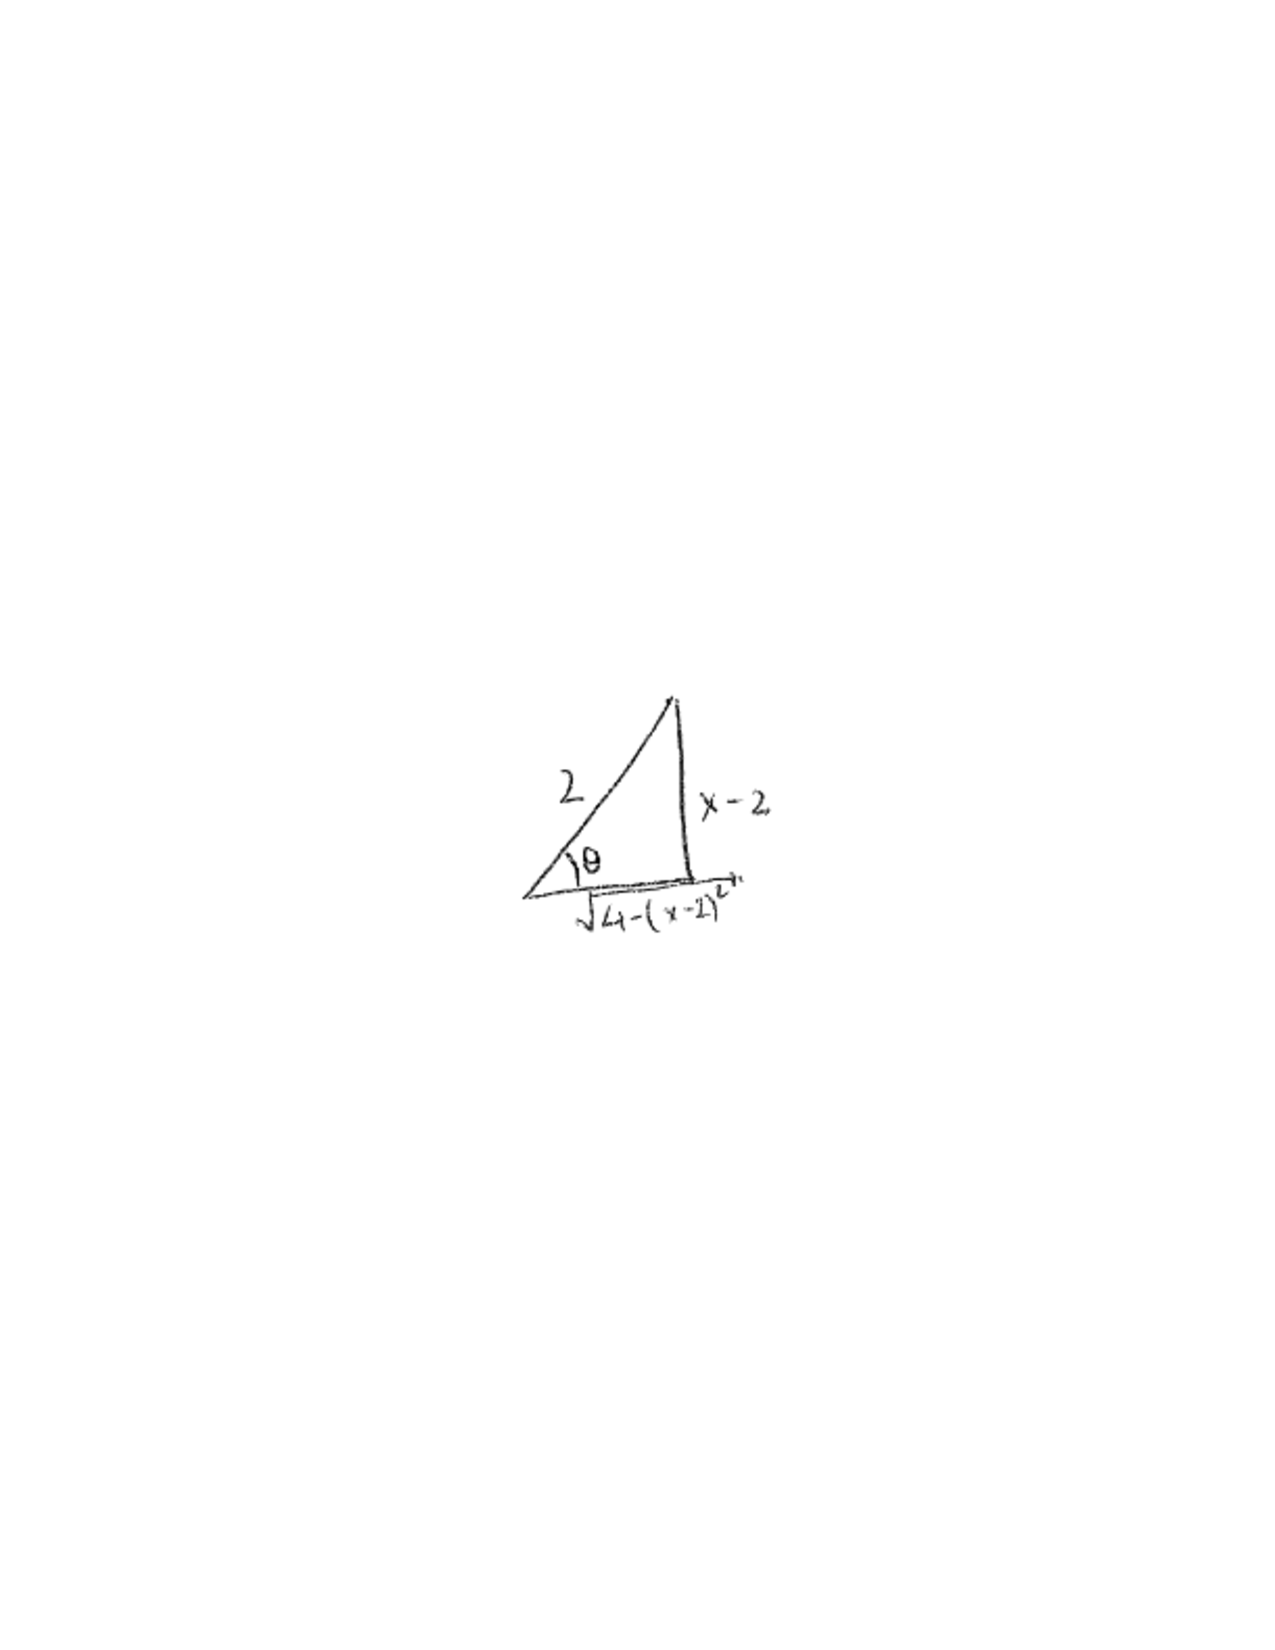
\includegraphics[trim= 270 350 250 330]{Figure7-4-2.pdf}
		\end{image}
		
	Then we have that
		\begin{align*}
		&\cos \theta = \frac{\sqrt{4-(x-2)^2}}{2}  \\
		&\sin(2\theta) = 2 \sin \theta \cos \theta = 2 \cdot \frac{x-2}{2} \cdot \frac{\sqrt{4-(x-2)^2}}{2}.
		\end{align*}
	Thus
		\[
		\int \frac{x^2}{\sqrt{4x-x^2}} \d x = 6\arcsin \left( \frac{x-2}{2} \right) - 4\sqrt{4-(x-2)^2} - \frac{(x-2)\sqrt{4-(x-2)^2}}{2}.
		\]
	\end{freeResponse}

	\item 
	\[
	\int \frac{e^x}{\sqrt{e^{2x}+9}} \d x.
	\]
	\begin{freeResponse}
	First, notice that
		\[
		\sqrt{e^{2x}+9} = \sqrt{9\left( \frac{e^{2x}}{9} + 1 \right)} = 3\sqrt{\left( \frac{e^x}{3} \right)^2 + 1}.
		\]
	So
		\[
		\int \frac{e^x}{\sqrt{e^{2x}+9}} \d x = \frac{1}{3} \int \frac{e^x}{\sqrt{\left( \frac{e^x}{3} \right)^2 + 1}} \d x.
		\]
	We make the substitution
		\begin{equation}\label{substitution3}
		\frac{e^x}{3} = \tan \theta 	\qquad	\Longrightarrow	\qquad	3\tan \theta = e^x
		\end{equation}
	which gives
		\[
		e^x \d x = 3 \sec^2 \theta \d \theta.
		\]
	Continuing with the integral, we have that
		\begin{align*}
		\frac{1}{3} \int \frac{e^x}{\sqrt{\left( \frac{e^x}{3} \right)^2 + 1}} \d x
		&= \frac{1}{3} \int \frac{1}{\sqrt{\tan^2 \theta + 1}} \cdot 3 \sec^2 \theta \d \theta  \\
		&= \int \sec \theta \d \theta  \\
		&= \ln | \sec \theta + \tan \theta | + C.
		\end{align*}
	Now all that is left to do is to reverse-substitute for $\theta$. 
	We use equation \eqref{substitution3} along with Pythagorean's Theorem to construct the following triangle.
	
		\begin{image}
		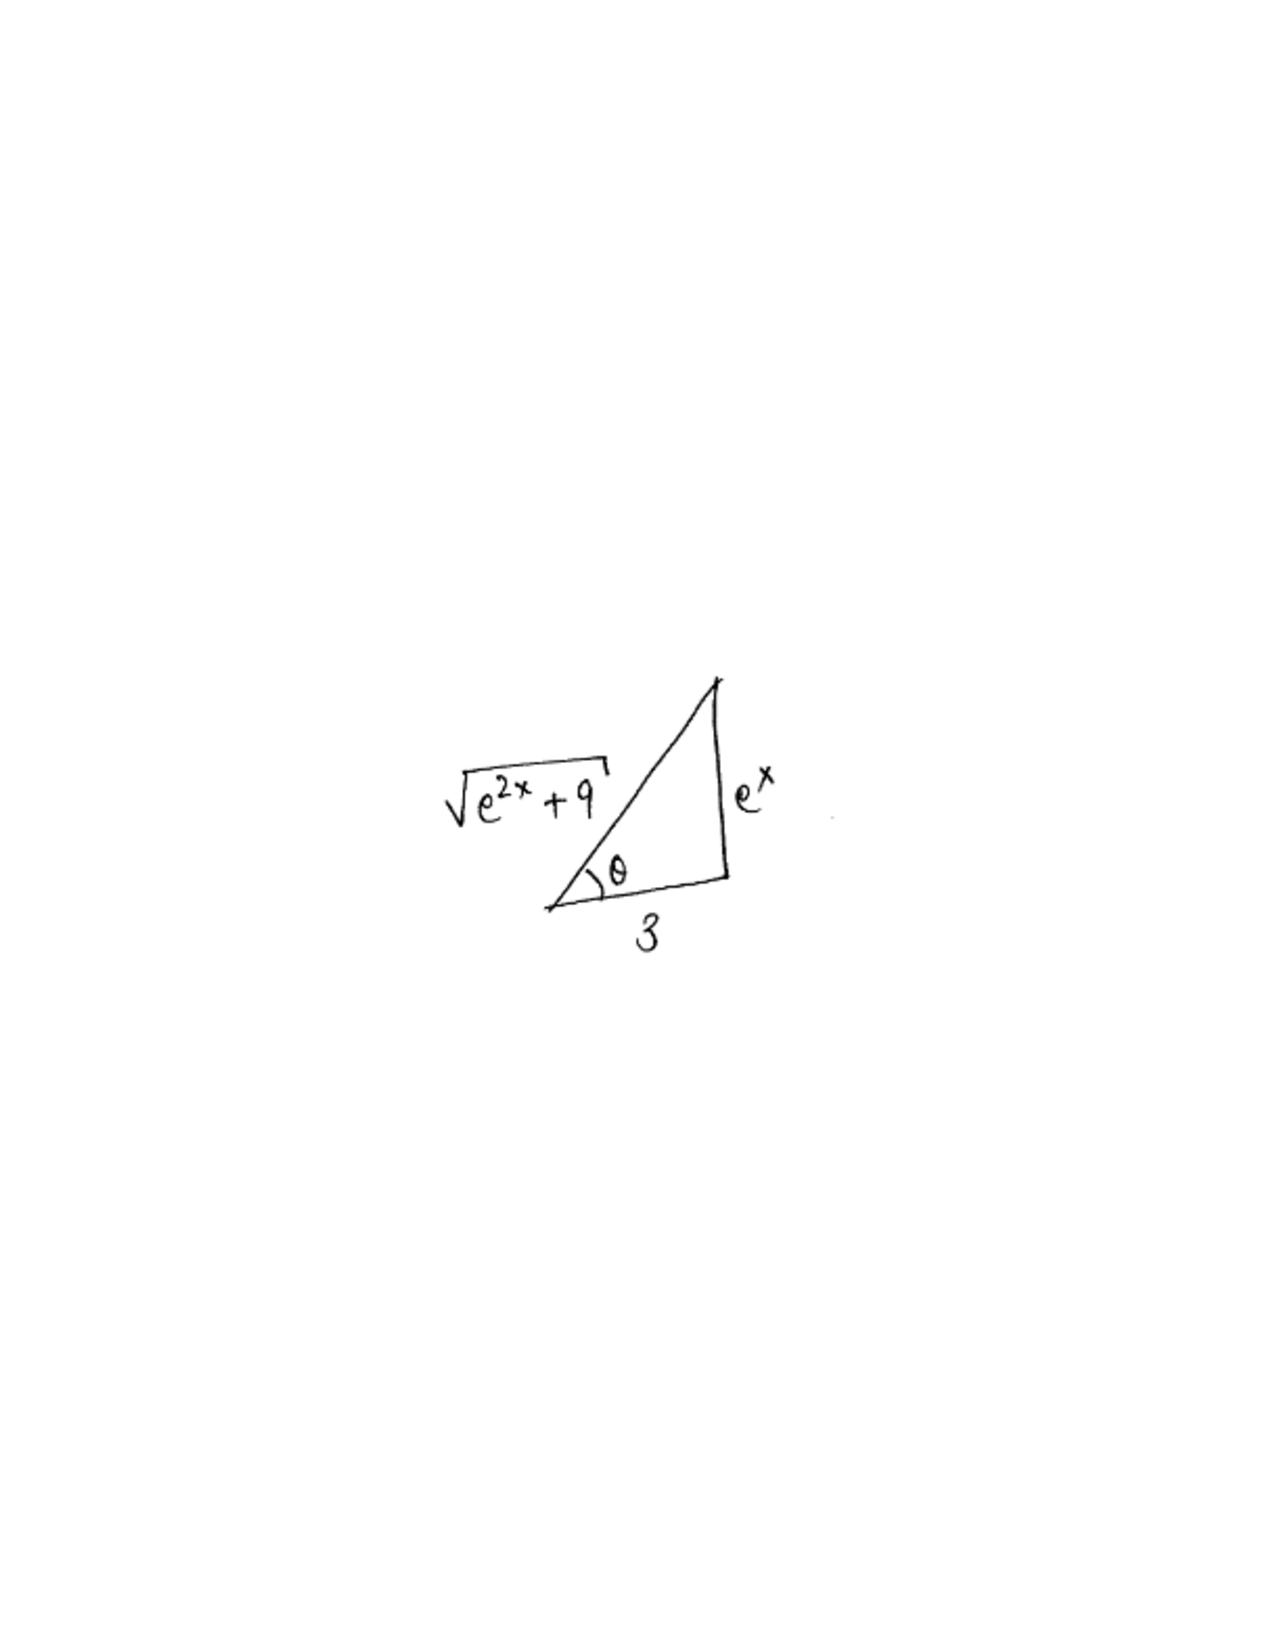
\includegraphics[trim= 270 350 250 330]{Figure7-4-3.pdf}
		\end{image}
		
	Then we have that
		\begin{align*}
		&\sec \theta = \frac{\sqrt{e^{2x}+9}}{3} \\
		&\tan \theta = \frac{e^x}{3}.
		\end{align*}
	Thus
		\[
		\int \frac{e^x}{\sqrt{e^{2x}+9}} \d x = \ln \left( \frac{\sqrt{e^{2x}+9} + e^x}{3} \right) + C.
		\]
	\end{freeResponse}



	\item 
	\[
	\int \frac{\d x}{x^{\frac{1}{2}} - 9x^{\frac{3}{2}}}.
	\]
	\begin{freeResponse}
		\begin{align*}
		\int \frac{\d x}{x^{\frac{1}{2}} - 9x^{\frac{3}{2}}}
		&= \int \frac{1}{x^{\frac{1}{2}} \left( 1 - 9x \right)} \d x  \\
		&= \int \frac{1}{x^{\frac{1}{2}} \left( 1 - \left( 3x^{\frac{1}{2}} \right)^2 \right)} \d x  \\
		&= \frac{2}{3} \int \frac{1}{1-u^2} \d x 	\qquad	{\color{red}\text{where }u=3x^{\frac{1}{2}}}  \\
		&= \frac{2}{3} \int \frac{1}{1-\sin^2 \theta} \cos \theta \d \theta	\qquad	{\color{red} \text{where } u=\sin \theta}  \\
		&= \frac{2}{3} \int \frac{\cos \theta}{\cos^2 \theta} \d \theta  \\
		&= \frac{2}{3} \int \sec \theta \d \theta  \\
		&= \frac{2}{3} \ln | \sec \theta + \tan \theta | + C  \\
		&= \frac{2}{3} \ln \left| \frac{1}{\sqrt{1-u^2}} + \frac{u}{\sqrt{1-u^2}} \right| + C  \\
		&= \frac{2}{3} \ln \left( \frac{1 + 3\sqrt{x}}{\sqrt{1-9x}} \right) + C
		\end{align*}
		
		\begin{image}
		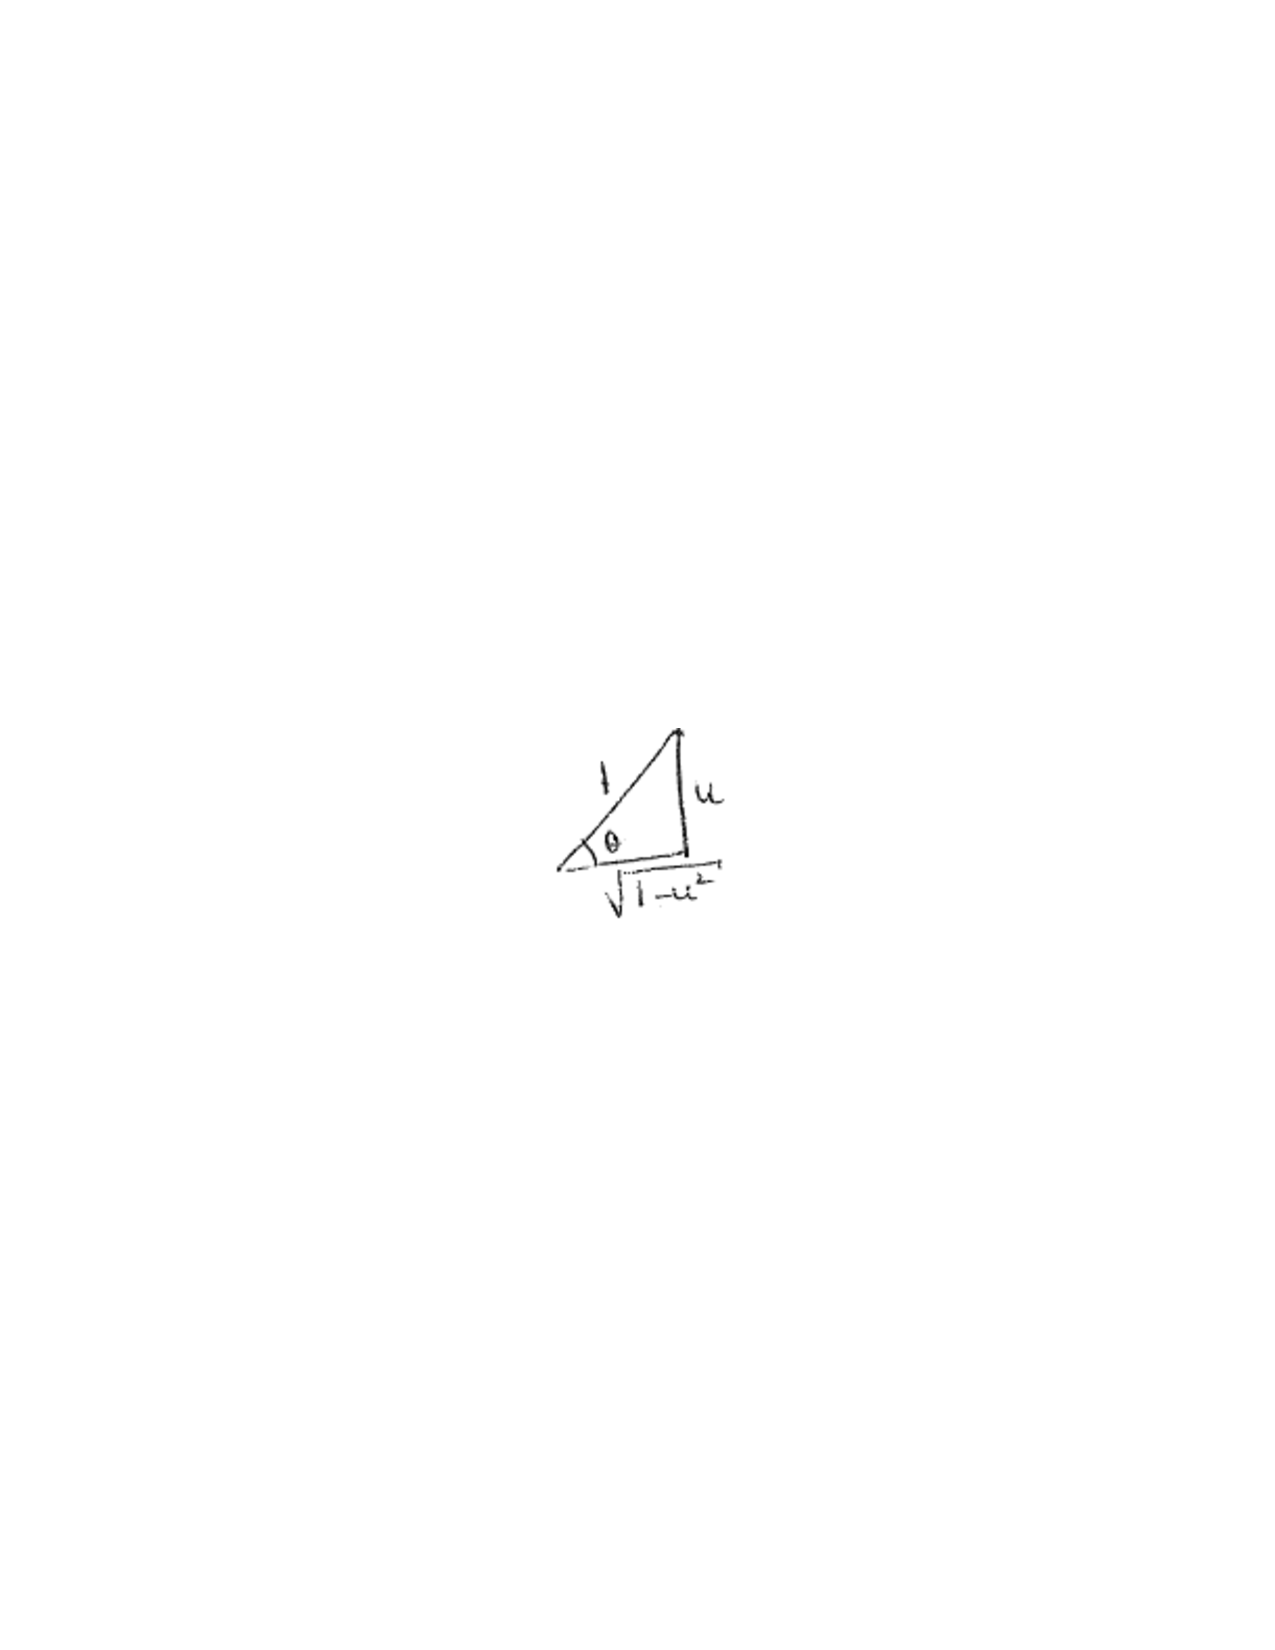
\includegraphics[trim= 270 350 250 360]{Figure7-4-4.pdf}
		\end{image}
		
	\end{freeResponse}

	\end{enumerate}

\end{problem}

\begin{instructorNotes}
Each of problems (a) through (c) involves one or more of the major points of trig substitution.  
Each of the three kinds of substitutions is represented, as well as working with absolute value issues in problem (a) (also could be brought up in problem (c)), completing the square, back substitution (c), and various trigonometric integrals.  
\dfn{Be adamant about substituting for $\d x$} as well as the rest of the integrand.  
In  (a), show the time-saving value of changing the limits in terms of $\theta$.  
\end{instructorNotes}












	
	
	
	
	
	
	
	
	

	










								
				
				
	














\end{document} 


















